%
% ---------- header -----------------------------------------------------------
%
% project       kaneton
%
% license       kaneton
%
% file          /home/texane/repo/kaneton/view/lecture/kernels/devices-new/devices-new.tex
%
% created       fabien le mentec
% updated       julien quintard   [wed apr 22 11:29:29 2009]
%

%
% ---------- setup ------------------------------------------------------------
%

%
% path
%

\def\path{../../..}

%
% template
%

%
% ---------- header -----------------------------------------------------------
%
% project       kaneton
%
% license       kaneton
%
% file          /home/mycure/kaneton/view/template/lecture.tex
%
% created       julien quintard   [wed may 16 18:17:26 2007]
% updated       julien quintard   [sun may 18 23:23:40 2008]
%

%
% class
%

\documentclass[8pt]{beamer}

%
% packages
%

\usepackage{pgf,pgfarrows,pgfnodes,pgfautomata,pgfheaps,pgfshade}
\usepackage[T1]{fontenc}
\usepackage{colortbl}
\usepackage{times}
\usepackage{amsmath,amssymb}
\usepackage{graphics}
\usepackage{graphicx}
\usepackage{color}
\usepackage{xcolor}
\usepackage[english]{babel}
\usepackage{enumerate}
\usepackage[latin1]{inputenc}
\usepackage{verbatim}
\usepackage{aeguill}

%
% style
%

\usepackage{beamerthemesplit}
\setbeamercovered{dynamic}

%
% verbatim stuff
%

\definecolor{verbatimcolor}{rgb}{0.00,0.40,0.00}

\makeatletter

\renewcommand{\verbatim@font}
  {\ttfamily\footnotesize\selectfont}

\def\verbatim@processline{
  {\color{verbatimcolor}\the\verbatim@line}\par
}

\makeatother

%
% -
%

\renewcommand{\-}{\vspace{0.4cm}}

%
% date
%

\date{\today}

%
% logos
%

\pgfdeclareimage[interpolate=true,width=34pt,height=18pt]
                {epita}{\path/logo/epita}
\pgfdeclareimage[interpolate=true,width=49pt,height=18pt]
                {upmc}{\path/logo/upmc}
\pgfdeclareimage[interpolate=true,width=25pt,height=18pt]
                {lse}{\path/logo/lse}

\newcommand{\logos}
  {
    \pgfuseimage{epita}
  }

%
% institute
%

\institute
{
  \inst{1} kaneton microkernel project
}

%
% table of contents at the beginning of each section
%

\AtBeginSection[]
{
  \begin{frame}<beamer>
   \frametitle{Outline}
    \tableofcontents[current]
  \end{frame}
}

%
% table of contents at the beginning of each subsection
%

\AtBeginSubsection[]
{
  \begin{frame}<beamer>
   \frametitle{Outline}
    \tableofcontents[current,currentsubsection]
  \end{frame}
}


%
% title
%

\title{Devices}

\usepackage{listings}
\usepackage{color}
\usepackage{verbatim}
\usepackage{graphicx}

%
% document
%

\begin{document}

%
% title frame
%

\begin{frame}
  \titlepage
\end{frame}

%
% outline frame
%

\begin{frame}
  \frametitle{Outline}

  \tableofcontents
\end{frame}

%
% Overview
%

\section{Overview}

% 1) contents

\begin{frame}
  \frametitle{Contents}

  This is course uses the guideline \textit{devices} as a pretext to cover the
  following topics
  \begin{itemize}
  \item device \textbf{communication}
  \item device \textbf{programming}
  \end{itemize}

\end{frame}


%
% Communication buses
%

\section{Device commnication}

\begin{frame}{General - Introduction}
  A device can be split into 2 parts
  \begin{itemize}
  \item the processing units controlling device specific mechanisms
    \begin{itemize}
    \item hard drive control mechanism
    \item PID controller for industrial processes
    \item robot engine controlling software
    \item sensor sampling software
    \end{itemize}
  \item a set of chips handling the \textbf{communication} logic
    \begin{itemize}
    \item signals: data, control, addressing, interrupt, power
    \item interface registers set
    \end{itemize}
  \end{itemize}

  \smallskip
  \begin{center}
    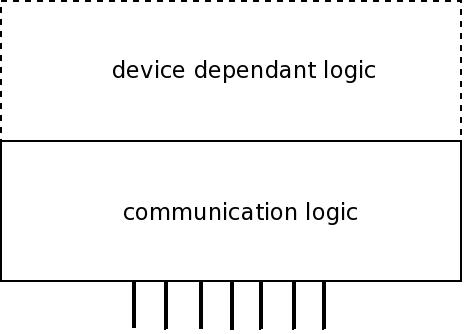
\includegraphics[width=0.3\textwidth]{figures/device_intro.jpg}
  \end{center}
\end{frame}

\begin{frame}{General - Introduction}
  Whenever information must be transmitted from one node to another in a global system,
  a communication scheme must be implemented. This is the role of \textbf{communication buses},
  or \textbf{networks}. Unless mentionned we use both terms equivalently.
\end{frame}

\begin{frame}{General - Introduction}
  Basically, communication is done by \textbf{interacting} with a medium
  \begin{itemize}
  \item transmiting is done by \textbf{altering} the medium
  \item receiving is done by \textbf{sensing} the medium variation
  \item devices are an \textbf{interface} with the medium
  \end{itemize}

  \smallskip
  Some examples
  \begin{itemize}
  \item most computer devices use \textbf{electrical field} variations to communicate
  \item a wireless network controller interacts with \textbf{electromagnetic field}
  \item ears and voice are devices used to interact with the air (\textbf{acoustics})
  \end{itemize}

\end{frame}

\begin{frame}{General - Communication criteria}
  Choosing an appropriate bus depends on several factors
  \begin{itemize}
  \item node \textbf{distance}
  \item \textbf{operating} environment (noise ...)
  \item communication \textbf{speed}
  \item \textbf{reliability} (realtime ...)
  \item \textbf{flexibility} (static addressing ...)
  \end{itemize}
\end{frame}

\begin{frame}{General - Transmission properties}
  Designing and implementing buses raises several issues for engineers and technicians.\\
  In general, those issues are solved by \textbf{layering} the problem.\\
  \begin{itemize}
  \item \textbf{physical} specifications (shape of connectors ...)
  \item \textbf{medium} specifications (voltage levels ...)
  \item \textbf{data} transmission (rs232 typical 9600 8N1 ...)
  \item supported \textbf{hardware mechanisms} (checksums, retries ...)
  \item bus \textbf{topology} (master/slave ...)
  \item node \textbf{addressing}
  \end{itemize}
\end{frame}

\begin{frame}{General - Transmission synchronism}
  A device controller must know at which moment to \textbf{sample} the bus.\\
  2 main schemes exist for determining this moment:
  \begin{itemize}
  \item \textbf{synchronous}
    \begin{itemize}
    \item nodes share a \textbf{clock signal}
    \item may have one clock per link
    \item may use both clock edges to increase bandwith
    \end{itemize}
  \item \textbf{asynchronous} (no clock shared)
    \begin{itemize}
    \item bus \textbf{frequency} is agreed upon
    \item mechanisms to take into account jittering, phases...
    \end{itemize}
  \item \textbf{hybrid}
    \begin{itemize}
    \item synchronous for initialization
    \item then asynchronous mode
    \end{itemize}
  \end{itemize}
\end{frame}

\begin{frame}{General - Transmission serialism}
  Bus signals can be organized in 2 ways
  \begin{itemize}
  \item \textbf{serial}
  \item \textbf{parallel}
  \end{itemize}

  \smallskip
  Intuitively, a parallel design allows for more bandwith. But at \textbf{high frequencies} and
  \textbf{small distances}, electrical constraints arise making serial links more efficient.
  \begin{itemize}
  \item at small distance, parallel signals can parasite each other
  \item at high frequency, small routing imprecisions become predominant
  \end{itemize}

  \smallskip
  For instance, PCIe switched from parallel to serial, USB links are serial...

  \smallskip
  \begin{center}
    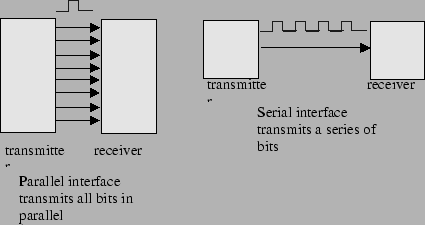
\includegraphics[width=0.4\textwidth]{figures/serial_parallel.png}
  \end{center}

\end{frame}

\begin{frame}{General - Network topologies}

  Network topologies is mostly a tradeoff between \textbf{flexibility} and \textbf{number of links}

  \smallskip
  \begin{center}
    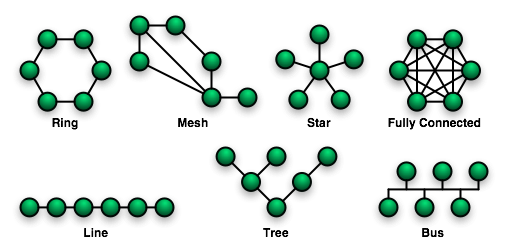
\includegraphics[width=0.5\textwidth]{figures/network_topo.png}
  \end{center}

  For instance, a \textbf{grid} decreases the number of links (compared with a fully connected topology)
  but introduces \textbf{non uniform transfer times} and \textbf{data routing complexity}.

\end{frame}

\begin{frame}{General - Buses to be covered}
  This course covers the the following communication buses

  \smallskip
  \begin{center}
    \begin{tabular}{|c|c|}
      \hline
      \textbf{Name} & \textbf{Reason} \\
      \hline
      CAN & standard \textbf{field} bus \\
      \hline
      USB &  standard PC \textbf{external} bus \\
      \hline
      PCIe & standard PC \textbf{internal} bus \\
      \hline
    \end{tabular}
    \smallskip
    \begin{tiny}
      \textit{\\Communication buses covered}
    \end{tiny}
  \end{center}

  It is likely you will develop \textbf{kernel drivers}, \textbf{userland libraries} or
  \textbf{VHDL cores} for some of them.

\end{frame}

\begin{frame}{General - More references}
  \begin{itemize}
  \item http://www.lintech.org/comp-per
  \end{itemize}
\end{frame}

% --- CAN

\begin{frame}{CAN - Motivations and Applications}
  Controller Area Network
  \begin{itemize}
  \item adding \textbf{determinism} and \textbf{realtime} to communications
  \item reducing the total \textbf{cable length} as the number of devices increases
  \item \textbf{2 wires} (plus an optionnal ground signal)
  \item \textbf{differential voltage} makes it more resistant to \textbf{noise}
  \item industrial plants, automotive industry
  \end{itemize}
\end{frame}


\begin{frame}{CAN - Transmission speeds versus distance}
  \begin{itemize}
  \item low speed CAN: up to 125Kb/s
  \item high speed CAN: 125Kb/s to 1Mb/s
  \end{itemize}

  \smallskip

  \begin{center}
    \begin{tabular}{|c|c|}
      \hline
      \textbf{Speed} (Kbits/s) & \textbf{Distance} (meters) \\
      \hline
      1024 & 60 \\
      500 & 150 \\
      100 & 1000 \\
      20 & 1200 \\
      \hline
    \end{tabular}
    \smallskip
    \begin{tiny}
      \textit{\\speed versus distance}
    \end{tiny}
  \end{center}

\end{frame}

\begin{frame}{CAN - Bit representation}
  In CAN terminology, a bit is considered either \textit{dominant} or \textit{recessive}.

  \begin{center}
    \begin{tabular}{|c|c|c|c|}
      \hline
      \textbf{terminology} & \textbf{logical} & \textbf{input voltage} & \textbf{output voltage} \\
      \hline
      dominant & 0 & 0.9v - 5.0v & 1.5v - 3.0v \\
      \hline
      recessive & 1 & -1.0v - 0.5v & -0.5v - 0.05v \\
      \hline
    \end{tabular}
    \smallskip
    \begin{tiny}
      \textit{\\CAN bit representations}
    \end{tiny}
  \end{center}

\end{frame}

\begin{frame}{CAN - Bit arbitration}
  \textbf{CSMA/BA}: Carrier sense multiple access/bitwise arbitration
  \begin{itemize}
    \item a \textbf{dominant} bit overdrives a \textbf{recessive} bit on the bus
    \item bitwise and operation, non destructive
    \item this is how \textbf{determinism} and \textbf{priority} are achieved
  \end{itemize}

  \smallskip
  \begin{center}
    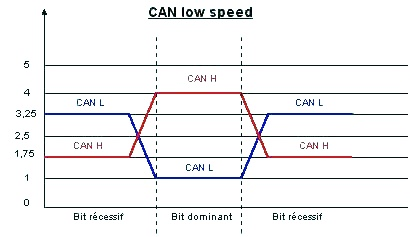
\includegraphics[width=0.5\textwidth]{figures/can_bit_lowspeed_levels.jpg}
    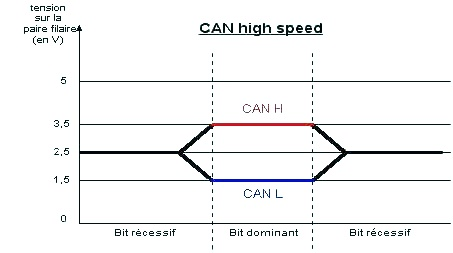
\includegraphics[width=0.5\textwidth]{figures/can_bit_highspeed_levels.jpg}
  \end{center}
\end{frame}

\begin{frame}{CAN - Bit timing}
  A bit is divided into 4 \textbf{time segments}
  \begin{itemize}
  \item synchronization, propagation, phase1, phase2
  \item the unit time is called the \textbf{time quanta}, Tq
  \item each segment is expressed in term of Tq (ie. sync == 2Tq ...)
  \item this model allows to take into account jitter, distance and various node latencies
  \item nodes clocks do not have to be the same, only Tq must correspond
  \end{itemize}

  \smallskip
  \begin{center}
    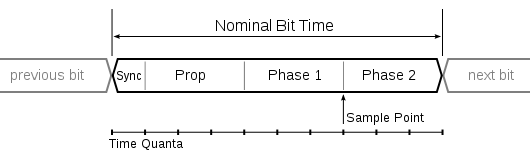
\includegraphics[width=0.7\textwidth]{figures/bit_timing.png}
  \end{center}
\end{frame}

\begin{frame}{CAN - Bit transmission}
  \begin{itemize}
  \item single ended, \textbf{Non Return to Zero} (NRZ)
  \item \textbf{bit stuffing} used to break successive bit chains
    \begin{itemize}
    \item a bit of \textbf{inversed polarity} is inserted every 5 \textbf{consecutive} bits
    \end{itemize}
  \end{itemize}

  \smallskip
  \smallskip
  \begin{center}
    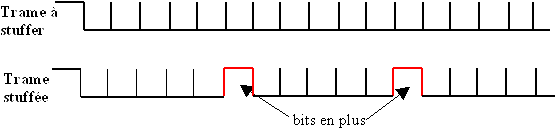
\includegraphics[width=0.7\textwidth]{figures/can_bit_stuffing.png}
  \end{center}
\end{frame}

\begin{frame}{CAN - Frame format}
  2 frame formats
  \begin{itemize}
  \item \textbf{standard} (CAN 2.0 A): 11 bits identifier
  \item \textbf{extended} (CAN 2.0 B): 29 bits identifier
  \end{itemize}

  \smallskip
  \begin{center}
    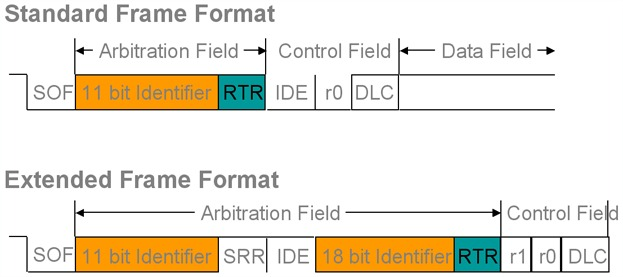
\includegraphics[width=0.7\textwidth]{figures/can_frame_format.jpg}
  \end{center}
\end{frame}

\begin{frame}{CAN - Frame types}
  4 different frame types
  \begin{itemize}
    \item \textbf{data}: containing payload data
    \item \textbf{remote}: request transmission of a specific identifier
    \item \textbf{error}: transmitted by a node detecting an error
    \item \textbf{bus overloaded}: inject a delay between data and remote frame
  \end{itemize}
\end{frame}

\begin{frame}{CAN - Node states}
  Node can transit from an error state to another
  \begin{itemize}
  \item 3 possible states
    \begin{itemize}
    \item \textbf{error active}
    \item \textbf{error passive}
    \item \textbf{bus off}
    \end{itemize}
  \item per node Rx et Tx error counters (TEC, REC)
  \end{itemize}

  \smallskip
  \begin{center}
    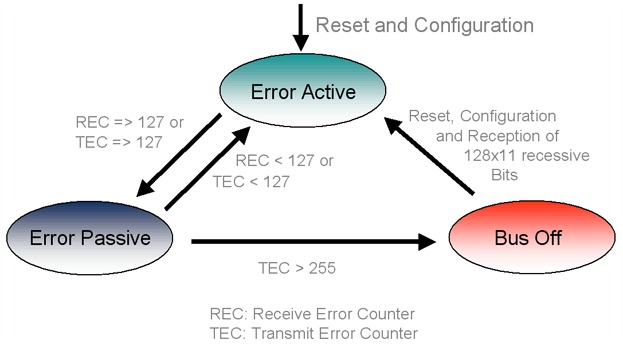
\includegraphics[width=0.5\textwidth]{figures/can_states.jpeg}
  \end{center}
\end{frame}

\begin{frame}{CAN - Robot communication network}
  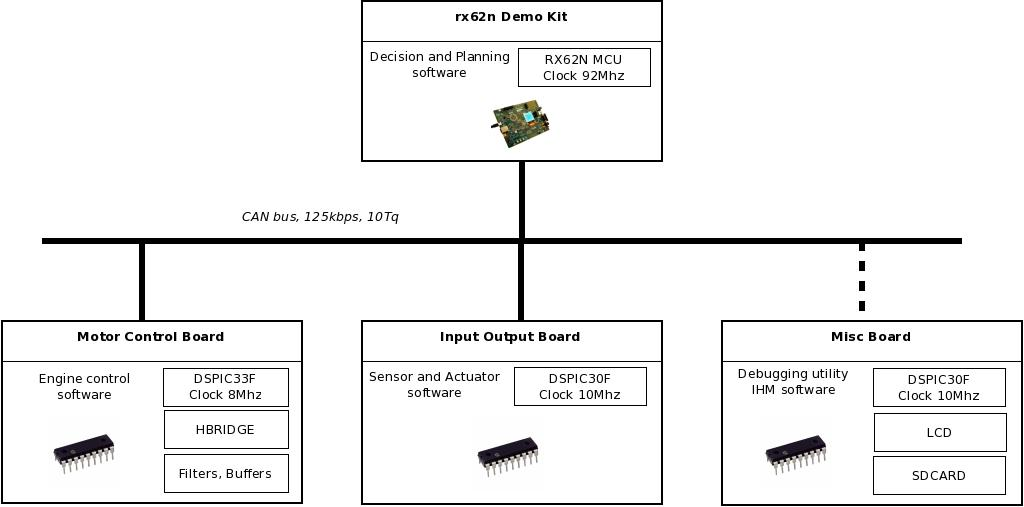
\includegraphics[width=\textwidth]{figures/igrebot_2011.jpg}
\end{frame}

\begin{frame}{CAN - References}
  \begin{itemize}
  \item http://uuu.enseirb-matmeca.fr/$\sim$kadionik/
  \item http://irisbachelard.free.fr/index.php?idPage=48
  \end{itemize}
\end{frame}
% --- CAN

% --- USB
\begin{frame}{USB - Overview}
  Universal Serial Bus. Typically used for external communication between
  host and devices.

  \begin{itemize}
  \item USB 1.1, 1998
    \begin{itemize}
    \item low speed, 1.5MBit/s
    \item full speed, 12 MBit/s
    \end{itemize}
  \item USB 2.0, 2000, High speed, 480 MBit/s
  \item USB 3.0, 2008, Super speed, 4.8 Gbit/s
  \end{itemize}

\end{frame}

\begin{frame}{USB - Topology}
  USB nodes are organized in an asymmetric, \textbf{tiered star} topology
  \smallskip
  \begin{center}
    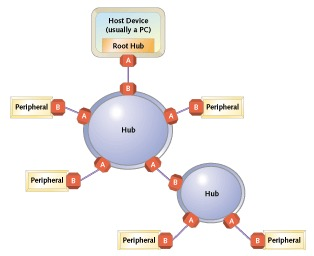
\includegraphics[width=0.4\textwidth]{figures/usb_topo.jpg}
  \end{center}
\end{frame}

\begin{frame}{USB - Concepts}
  \begin{itemize}
  \item communication relies on logical channels called \textbf{pipes}
  \item a pipe connects device and host controller \textbf{endpoints}
    \begin{itemize}
    \item a stream pipe is an \textbf{unidirectionnal} pipe for \textbf{data} transfer
    \item a message pipe is a \textbf{bidirectionnal} pipe used for \textbf{control}
    \end{itemize}
  \item there is a maximum of 32 endpoints per device (16 in, 16 out)
    \begin{itemize}
    \item endpoint 0 must be implemented and is reserved for configuration
    \item endpoints have a direction
    \end{itemize}
  \item \textbf{host centric}, \textbf{polled} bus
    \begin{itemize}
    \item any transfer is initiated by the host
    \item ease the communcation design
    \end{itemize}
  \end{itemize}
  \begin{center}
    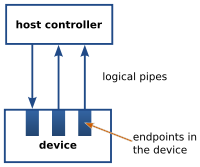
\includegraphics[width=0.2\textwidth]{figures/usb_host_dev.png}
  \end{center}
\end{frame}

\begin{frame}{USB - Device descriptors}
  Devices have a \textbf{descriptor hierarchy} containing configuration and operating information
  \smallskip
  \begin{center}
    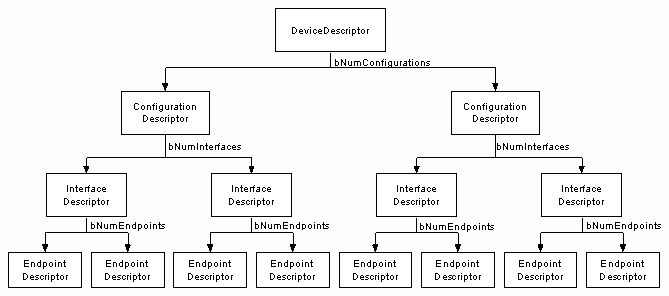
\includegraphics[width=0.9\textwidth]{figures/usb_desc_tree.jpg}
  \end{center}
\end{frame}

\begin{frame}{USB - Pinout}
  5V differential asynchronous serial link
  \smallskip
  \begin{center}
    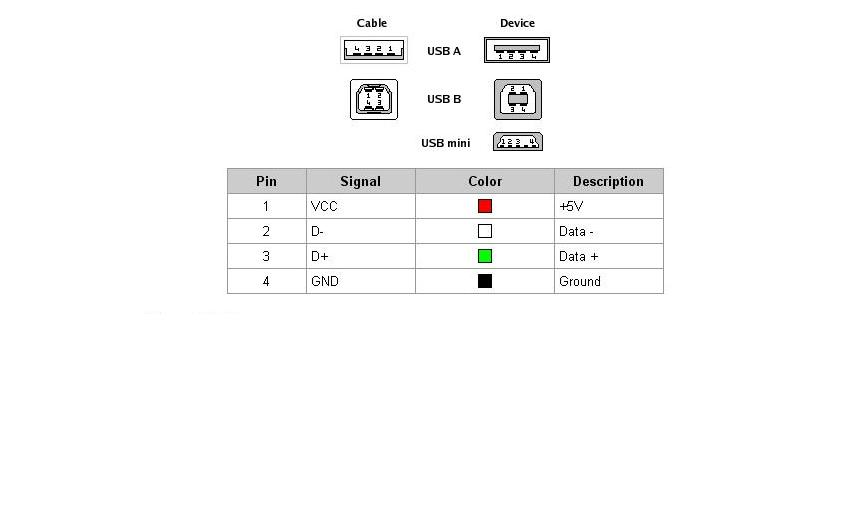
\includegraphics[width=0.8\textwidth]{figures/usb_pinout.jpg}
  \end{center}
\end{frame}

\begin{frame}{USB - Transfer modes}
  USB covers a wide panel of devices, some having conflicting requirements.
  \begin{itemize}
  \item for a mice, \textbf{data loss} is acceptable as it improves \textbf{latency}
  \item for a mass storage, \textbf{large payloads} are considered and \textbf{reliability} is a priority
  \item for a webcam, \textbf{large payloads} are considered but \textbf{realtime} is the priority
  \end{itemize}

  \smallskip
  Several transfer modes are thus available:
  \smallskip
  \begin{center}
    \begin{tabular}{|c|c|c|}
      \hline
      \textbf{Terminology} & \textbf{Description} & \textbf{Usage} \\
      \hline
      control & status commands & configuration, initialisation \\
      \hline
      interrupt & low latency, small payload & keyboards \\
      \hline
      isochronous & guaranteed bandwidth, large payload & audio, video \\
      \hline
      bulk & reliability, maximize bandwidth & file transfers \\
      \hline
    \end{tabular}
    \smallskip
    \begin{tiny}
      \textit{\\USB transfer types}
    \end{tiny}
  \end{center}
\end{frame}

\begin{frame}{USB - Addressing}
  Endpoints are addressable via a <\textbf{device\_address}, \textbf{endpoint\_number}> tuple
  \begin{itemize}
  \item endpoint\_number limited to 128
  \end{itemize}
\end{frame}

\begin{frame}{USB - Packet types}
  \begin{center}
    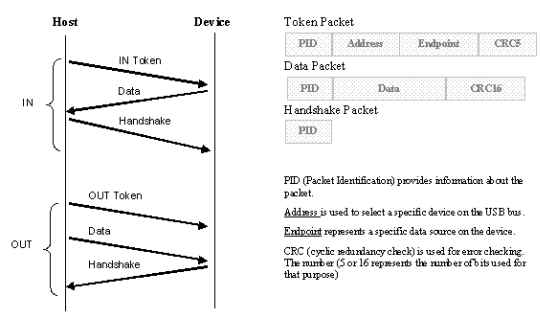
\includegraphics[width=0.75\textwidth]{figures/usb_packet.png}
  \end{center}
\end{frame}

\begin{frame}{USB - NRZI encoding}
  Non Return to Zero Invert
  \begin{itemize}
  \item 1 is represented by no change in voltage level
  \item 0 is represented a change in voltage level
  \end{itemize}

  \smallskip
  \begin{center}
    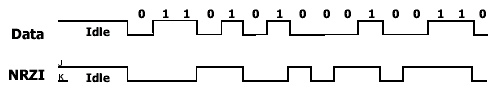
\includegraphics[width=0.8\textwidth]{figures/usb_nrzi.jpg}
  \end{center}

  Bit stuffing used to break chains of 6 consecutive 1s

\end{frame}

\begin{frame}{USB - Building your own devices}
  \begin{itemize}
  \item MICROCHIP PIC18F2550 has a USB module
    \begin{itemize}
    \item http://www.microchip.com
    \end{itemize}
  \item VASCO PUF framework provides an opensource USB stack for PICs
    \begin{itemize}
    \item http://vasco.gforge.enseeiht.fr
    \end{itemize}
  \item PINGUINO is a project using both of them
    \begin{itemize}
    \item http://www.hackinglab.org
    \end{itemize}
  \end{itemize}

  \smallskip
  \begin{center}
    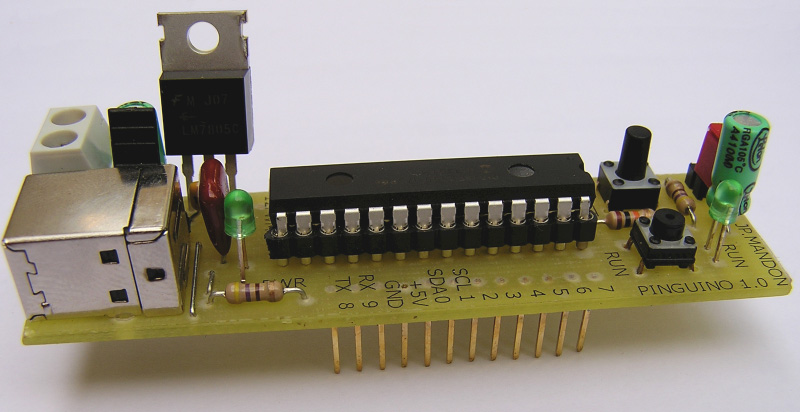
\includegraphics[width=0.6\textwidth]{figures/pinguino.jpg}
  \end{center}

\end{frame}

\begin{frame}{USB - References}
  \begin{itemize}
  \item http://www.usb.org
  \item http://www.beyondlogic.org/usbnutshell
  \end{itemize}
\end{frame}

% --- USB

% --- PCIe
\begin{frame}{PCIe - Overview}
  Peripheral Component Interconnect. Typically used for internal communication
  between host and devices.
\end{frame}

\begin{frame}{PCIe - HPC machine at INRIA}
  \begin{center}
    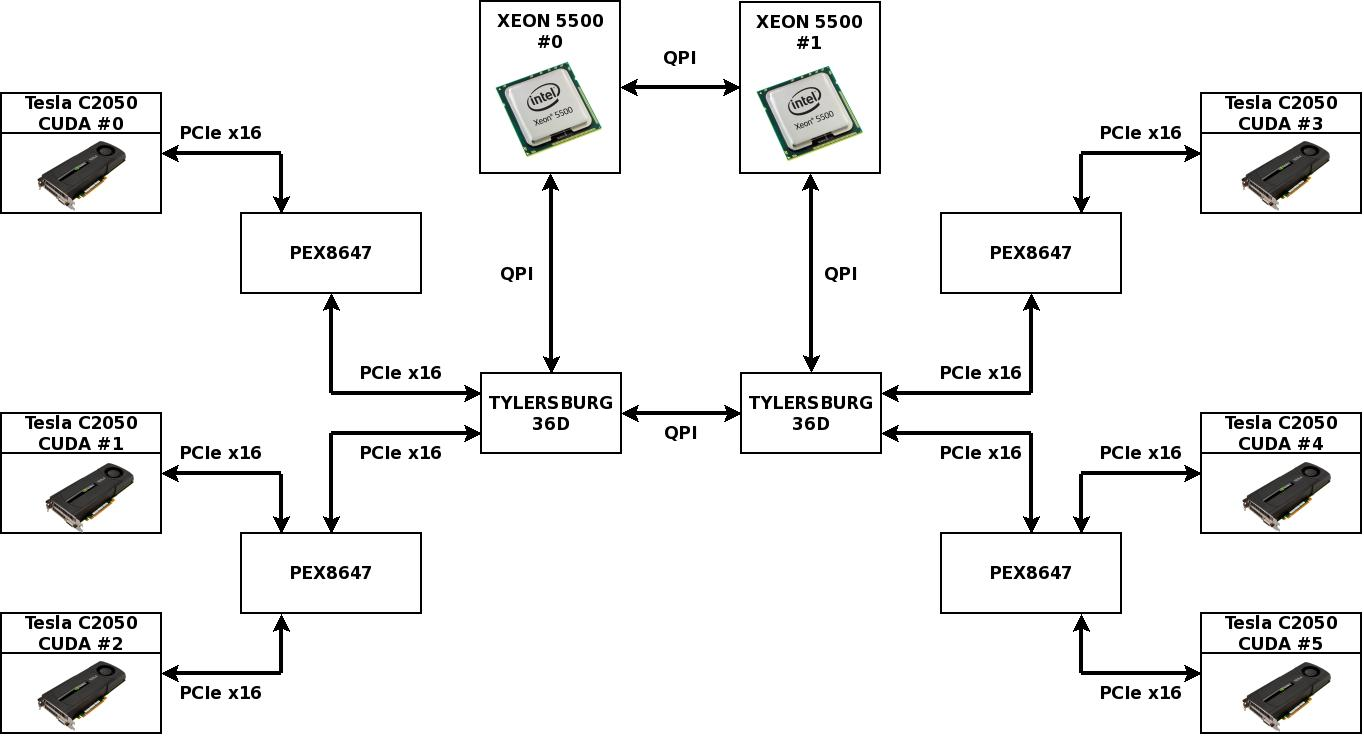
\includegraphics[width=0.9\textwidth]{figures/idgraph_bus_topo.jpg}
  \end{center}
\end{frame}

\begin{frame}{PCIe - Characteristics}
  \begin{itemize}
  \item \textbf{bidirectionnal} \textbf{serial}, \textbf{point to point} links
  \item 500 MB/s per lane with PCIe v2
  \item a lane is a \textbf{full-duplex} byte (8 bits) stream
  \item each slot can have up to 16 lanes
  \item a slot can have less connected lanes than physically possible
  \end{itemize}
\end{frame}

\begin{frame}[containsverbatim]{PCIe - Addressing}
  <\textbf{bus}:8>:<\textbf{device}:5>.<\textbf{function}:3>
  \begin{itemize}
  \item bus: multiple bus possible, bridged topology 
  \item device: the physical unit (ie. multimedia card)
  \item function: the actual processing unit (ie. graphics, audio)
  \end{itemize}

  \smallskip
\begin{verbatim}
00:1d.0 USB Controller [0c03]:USB UHCI Controller #1 [8086:27c8]
00:1d.1 USB Controller [0c03]:USB UHCI Controller #2 [8086:27c9]
00:1d.2 USB Controller [0c03]:USB UHCI Controller #3 [8086:27ca]
00:1d.3 USB Controller [0c03]:USB UHCI Controller #4 [8086:27cb]
00:1d.7 USB Controller [0c03]:USB2 EHCI Controller [8086:27cc]
\end{verbatim}

\end{frame}

\begin{frame}{PCIe - Configuration Space}
  A PCI compatible device exposes a 256 bytes \textbf{configuration space}
  \begin{itemize}
  \item 64 bytes well structured, followed by vendor specific 192 bytes
  \item \textbf{Base Address Registers} contains the assigned device address
  \end{itemize}

  \begin{center}
    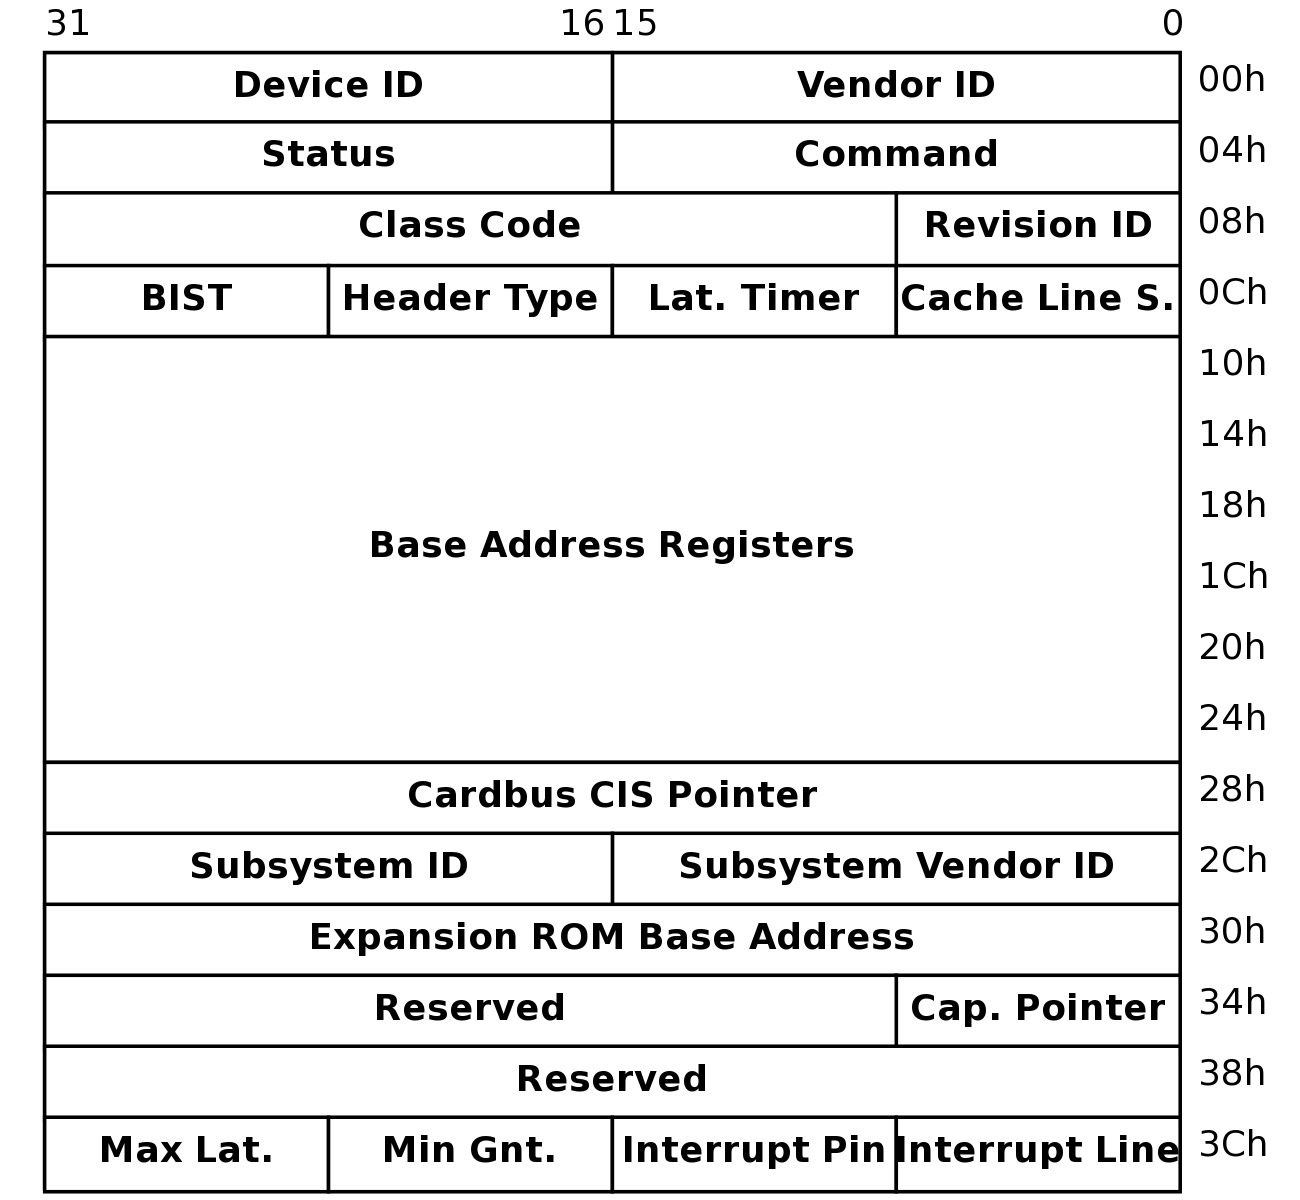
\includegraphics[width=0.4\textwidth]{figures/pci_config_space.jpg}
    \smallskip
    \begin{tiny}
      \textit{\\PCI Configuration Space}
    \end{tiny}
  \end{center}

\end{frame}

%% TODO
%% \begin{frame}{PCIe - Enumeration protocol}
%% \end{frame}

\begin{frame}{PCIe - References}
  \begin{itemize}
  \item http://www.pcisig.com
  \item http://www.interfacebus.com/PCI-Express-Bus-PCIe-Description.html
  \end{itemize}
\end{frame}

% --- PCIe

% --- Others
\begin{frame}{Other buses you may encounter}
  \begin{itemize}
  \item high speed: QuickPath Interconnect, HyperTransport
    \begin{itemize}
    \item 32 high speed point to point links (up to 3.2ghz)
    \item 25.6 GB/s. per direction
    \end{itemize}
  \item embeded: I2C, SPI
  \end{itemize}
\end{frame}
% --- Others

%
% Devices programming
%
\section{Device programming}

% specifications
\begin{frame}{Device specifications - Overview}
  There is a typical \textbf{documentation set} associated with a device
  \begin{itemize}
  \item device \textbf{datasheet}
    \begin{itemize}
    \item physical specifications
    \item electrical specifications
    \item expected operating environment
    \item timing diagrams
    \item programming interface
  \end{itemize}
  \item \textbf{application notes}
  \item \textbf{erratums}
  \end{itemize}
\end{frame}

\begin{frame}{Device specifications - Physical specifications}
  Dimensionnal characteristics of the device parts
  \begin{itemize}
  \item connector layouts
  \item case dimensions
  \item screw references
  \end{itemize}
\end{frame}

\begin{frame}{Device specifications - Electrical specifications}
  Operating voltage of the device
  \begin{itemize}
  \item operating voltages (ie. TTL, CMOS ...)
  \item operating frequency (ie. gain versus frequency)
  \end{itemize}
\end{frame}

\begin{frame}{Device specifications - Operating environment}
  The vendor gives warranties of \textbf{correctness} for \textbf{operating ranges}
  \begin{itemize}
  \item cutoff frequencies (ie. frequency versus amplification ...)
  \item environmental factors (ie. accuracy versus temperature, humidity, pressure ...)
  \end{itemize}
\end{frame}

\begin{frame}{Device specifications - Timing diagrams}
  \begin{center}
    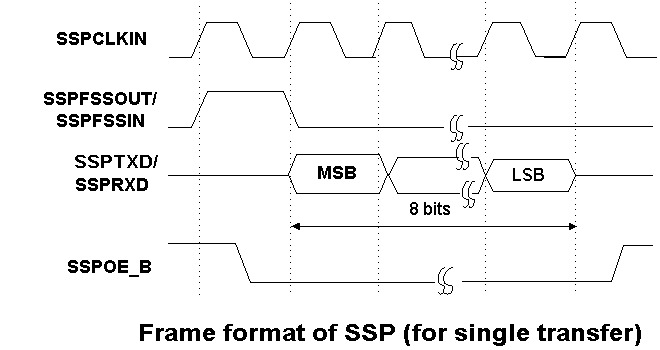
\includegraphics[width=0.5\textwidth]{figures/misc_timing.jpg}
  \end{center}
\end{frame}

\begin{frame}{Device specifications - Programming specifications}
  Any device exposes its programming interface as a set of programmable registers
  \begin{itemize}
  \item \textbf{control}: device operating mode ...
  \item \textbf{data}: fifo buffers ...
  \item \textbf{interrupt}: interrupt mask, status ...
  \item \textbf{error}: missed rx frames count ...
  \item \textbf{statistics}: L2 cache miss count ...
  \end{itemize}
\end{frame}

\begin{frame}{Device specifications - Application notes}
  Application notes show how to use the device in a typical application.
\end{frame}

\begin{frame}{Device specifications - Erratums}
  This is a set of bugs discovered post fabrication. Generally, a new device \textbf{revision}
  fixes the listed bugs. Taking a look at this file \textbf{early} in the development process
  can save the developper a lot of time.
\end{frame}

% programming
\begin{frame}{Device programming - Developper situation}
  A device developer is in one of the following cases
  \begin{itemize}
  \item she has the \textbf{device datasheets} only
  \item she is provided with a \textbf{driver} (with or without source code)
  \item she has a \textbf{driver} and a userland \textbf{library}
  \end{itemize}
\end{frame}

\begin{frame}{Device programming - Accessing register}
  Accessing the device registers is \textbf{architecture dependant}. 2 typical access schemes:
  \begin{itemize}
  \item \textbf{memory mapped} IOs: conventional load and store
    \begin{itemize}
    \item physical address trapped by a bus bridge, not forwarded to the RAM controller
    \end{itemize}
  \item \textbf{special purpose} instructions: IA32 has \textbf{in} and \textbf{out} instructions
  \end{itemize}
\end{frame}

\begin{frame}{Device programming - Notes on memory mapped IOs}
  \begin{itemize}
  \item memory mapped accesses should bypass the \textbf{cache hierarchy}
    \begin{itemize}
    \item page table attributes and MTRRs on IA32
    \end{itemize}
  \item pointer should be declared \textbf{volatile} to prevent compiler optimization
  \item bus requests may need to be \textbf{aligned} and of a given \textbf{width}
  \item possible to do access from userland (\textit{/dev/mem} mapping)
  \end{itemize}
\end{frame}

\begin{frame}[containsverbatim]{Programming device - /dev/mem example}
  \begin{tiny}
    \lstset{commentstyle=\color{blue}}
    \lstset{language=C}
    \begin{lstlisting}[frame=tb]
/* The SBC2410 kit ARM9 datasheet tells you:
 * . the I2C controller mapping starts at 0x56000000
 * . I2C control register starts at offset 0x50
 * . I2C data register starts at offset 0x54
 */

#define REGBASE 0x56000000
#define GPFCON 0x50
#define GPFDAT 0x54
#define GPFUP  0x58

typedef struct i2c_dev {
  int fd;
  unsigned char* base;
  volatile uint32_t* gpfconptr;
  volatile uint32_t* gpfdatptr;
} i2c_dev_t;

/* mapping the device */
dev->fd = open("/dev/mem", O_RDWR | O_SYNC);
dev->base = mmap(0, MAP_SIZE, PROT_READ | PROT_WRITE, MAP_SHARED, dev->fd, REGBASE);

/* take care of affecting volatile  pointers
 * accesses are done on a 32 bit width basis
 */
dev->gpfdatptr = (volatile uint32_t*)(dev->base + GPFDAT);
dev->gpfconptr = (volatile uint32_t*)(dev->base + GPFCON);

/* registers can be accessed through conventionnal load and store instructions
 */
*dev->gpfconptr = 0xdeadbeef;
uint32_t my_data = *dev->gpfdatptr;
    \end{lstlisting}
  \end{tiny}
\end{frame}

\begin{frame}{Device programming - Interrupts versus polling}
  When the CPU has to know about a device related event status, it can:
  \begin{itemize}
  \item regularly \textbf{poll} the device registers
  \item be \textbf{notified} by the device
  \end{itemize}

  Notifications are sent by the device through one or more \textbf{interrupt lines}.
  Typically, the hardware has an \textbf{interrupt unit} containing an address vector
  for jumping on a \textbf{service routine} upon interrupt reception.

  \smallskip
  \begin{center}
    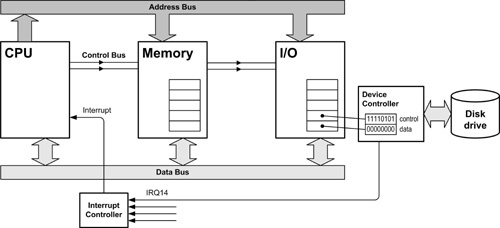
\includegraphics[width=0.5\textwidth]{figures/misc_irq.jpg}
  \end{center}

\end{frame}

\begin{frame}{Device programming - Memory transfers}
  \textbf{Direct Memory Access} (DMA) is used to perform asynchronous memory transfers
  \begin{itemize}
  \item host to device
  \item device to host
  \item device to device
  \end{itemize}

  \smallskip
  \begin{center}
    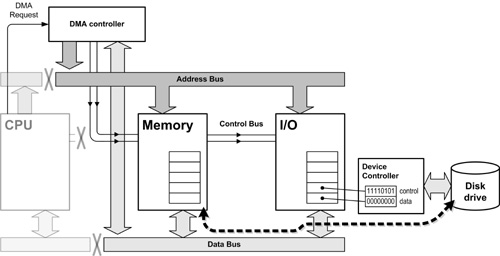
\includegraphics[width=0.5\textwidth]{figures/misc_dma.jpg}
  \end{center}
\end{frame}

\begin{frame}{Device programming - Software}
  Mainly 3 software layers

  \begin{itemize}
  \item \textbf{kernel driver} model
    \begin{itemize}
    \item Windows NT driver model (IO stacks and message passing between the stack nodes)
    \item Linux driver ``model'' (not unified, function based but USB subsystem relies on URB...)
    \end{itemize}

  \item \textbf{file interface} or \textbf{object model}
    \begin{itemize}
    \item stands on top of the kernel
    \item LINUX: open, close, read, write, ioctl
    \item WINDOWS NT: NtXxxFile routines family
    \end{itemize}

  \item \textbf{API}
    \begin{itemize}
    \item example: LIBUSB
    \end{itemize}

  \end{itemize}

\end{frame}

\begin{frame}{Device programming - Development process}
  There are typical steps for programming a device driver
  \begin{itemize}
  \item documentation
    \begin{itemize}
    \item architecture and device datasheets, erratums
    \item understand the processor architecture (esp. operating frequency, interrupt handling)
    \item understand the device (esp. associated state transition)
    \end{itemize}
  \item implementation
    \begin{itemize}
    \item modify existing source code (ie. from application notes)
    \item implement from scratch
    \end{itemize}
  \item testing
    \begin{itemize}
    \item functionnal (are the nodes properly communicating)
    \item environmental (put the device near electromag sources)
    \item performance (actual versus peak bandwith)
    \item stress (packet loss handling)
    \item robustness (put the device into unexpected situations)
    \end{itemize}
  \end{itemize}
\end{frame}

\begin{frame}{Device programming - Reversing}
  Lack of doucmentation may lead you to find out by yourself. \textbf{Sniffing tools} are a good
  place to start (when traffic not encrypted):
  \begin{itemize}
  \item software api level: usbmon, detour library on WINDOWS...
  \item monitor PCI accesses: DIOT, IOMM
  \item hardware logic analyzer: bus pirate
  \item any digital oscilloscope (but frequency limits...)
  \end{itemize}
\end{frame}

%
% Questions
%

\section{Questions}
\begin{frame}
  \begin{center}
    QUESTIONS
  \end{center}
\end{frame}

\end{document}
